%%%%%%%%%%%%%%%%%%%%%%%%%%%%%%%%%%%%%%%%%%%%%%%%%%%%%%%%%%%%%%%%%%%%%%%%
% Escuela Politécnica Superior de la Universidad de Alicante
% Realizado por: Jose Manuel Requena Plens
% Contacto: info@jmrplens.com / Telegram:@jmrplens
%%%%%%%%%%%%%%%%%%%%%%%%%%%%%%%%%%%%%%%%%%%%%%%%%%%%%%%%%%%%%%%%%%%%%%%%

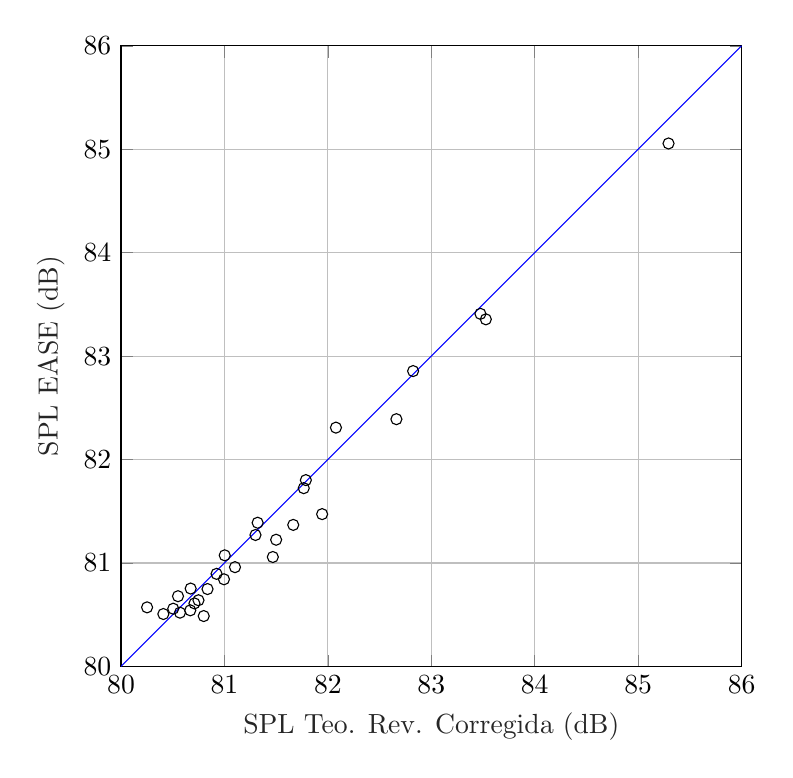
\begin{tikzpicture}

\begin{axis}[%
width=\textwidth,
height=0.65\textwidth,
at={(0\textwidth,0\textwidth)},
scale only axis,
xmin=80,
xmax=86,
xlabel style={font=\color{white!15!black}},
xlabel={SPL Teo. Rev. Corregida (dB)},
ymin=80,
ymax=86,
axis equal image=true,
%minor x tick num= 1,
%minor y tick num= 1,
%ytick distance=0.1,
ylabel style={font=\color{white!15!black}},
ylabel={SPL EASE (dB)},
axis background/.style={fill=white},
xmajorgrids,
xminorgrids,
ymajorgrids,
yminorgrids,
legend style={legend cell align=left, align=left, draw=white!15!black}
]
\addplot [color=black, only marks, mark=o]
  table[row sep=crcr]{%
80.6697126771525	80.5417995751689\\
88.3808391236599	88.7851487031814\\
80.5700129654216	80.5194381653846\\
80.2520438800622	80.5705747971496\\
80.5508547076089	80.6784606261286\\
80.9954788950488	80.8419021658868\\
81.0025149070337	81.0737051824391\\
81.3208054322234	81.3888549885737\\
81.7870262070404	81.8009255328463\\
82.0778955814787	82.3083613756488\\
82.8240090793044	82.8552558916018\\
80.7098929463617	80.6089698668838\\
83.5272045055965	83.3555043332764\\
80.7996545494746	80.4865223187322\\
80.4092875811931	80.5062700575210\\
80.5048862291226	80.5575264261869\\
80.7488175613742	80.6393766770917\\
80.6731668471498	80.7525117136745\\
80.9235270091036	80.8945590935560\\
81.4677403312375	81.0574750372379\\
81.4997990721067	81.2243740808657\\
81.6650826299988	81.3679913557655\\
80.8362954223367	80.7475438872565\\
81.9443544059675	81.4720812987855\\
81.1018723483650	80.9592620115112\\
81.2999367072749	81.2703621517406\\
81.7665926486219	81.7230177407061\\
82.6625494089014	82.3900472787150\\
83.4748783371691	83.4086834488246\\
85.2936795349521	85.0558095090494\\
};

\addplot [blue,samples at={80,86}] {x};
\end{axis}
\end{tikzpicture}%